\newpage
\section{Approssimazione di Integrali Definiti (Formule di Quadratura)}
\subsection{Formule di Newton-Cotes}
Il problema è il calcolo di integrali definiti:
\begin{equation}
I(f) = \int_{a}^{b} f(x) dx
\end{equation}
Assumeremo che $f \colon [a,b] \to \mathbb{R}$, con $f \in C([a,b])$, in modo che l'integrale esista nel senso classico. Per lo stesso motivo, assumeremo $-\infty < a < b < +\infty$.

Nel caso in cui la primitiva di $f(x)$ sia non nota o difficile da calcolare, si ricorre ad un opportuno metodo numerico. In generale, si approssimerà:
\begin{equation}
I(f) \approx \int_{a}^{b} p(x) dx, \quad \text{dove } p(x) \approx f(x)
\end{equation}
Chiaramente, ricercheremo $p(x)$ in una classe di funzioni per le quali il calcolo della primitiva sia semplice. Sicuramente, i polinomi sono tra queste. 
Nel caso specifico consideriamo il polinomio $p(x)$ di grado $n$ che interpola $f(x)$ sulle $n+1$ ascisse equidistanti:
\begin{equation} \label{eq:nodi_equidistanti}
x_i = a + ih, \quad i=0, \dots, n \quad \text{con } h = \frac{b-a}{n}
\end{equation}

Vediamo di derivare questo metodo, che definisce la \textbf{formula di Newton-Cotes di grado $n$}, che denoteremo con $I_n(f)$.
Si ottiene che, se $p(x) \in \Pi_n$ e $p(x_i) = f(x_i) \equiv f_i$ per $i=0, \dots, n$:
\begin{align*}
I_n(f) &= \int_{a}^{b} p(x) dx = \int_{a}^{b} \sum_{i=0}^{n} f_i L_{in}(x) dx \\
&= \sum_{i=0}^{n} f_i \int_{a}^{b} L_{in}(x) dx \quad (*)
\end{align*}

Inoltre, ricordando la definizione dei polinomi base di Lagrange:
\begin{equation*}
\int_{a}^{b} L_{in}(x) dx = \int_{a}^{b} \prod_{\substack{j=0 \\ j \neq i}}^{n} \frac{x - x_j}{x_i - x_j} dx
\end{equation*}
Operiamo la trasformazione $x = a + th \implies dx = h dt$. I limiti di integrazione diventano $t \in [0, n]$, e tenendo conto che $x_j = a + jh$:
\begin{equation*}
= h \int_{0}^{n} \prod_{\substack{j=0 \\ j \neq i}}^{n} \frac{a + th - (a + jh)}{a + ih - (a + jh)} dt = h \int_{0}^{n} \prod_{\substack{j=0 \\ j \neq i}}^{n} \frac{t - j}{i - j} dt \equiv h \cdot c_{in}
\end{equation*}
Pertanto, dalla $(*)$ otteniamo che:
\begin{equation} \label{eq:formula_newton_cotes}
I_n(f) = \frac{b-a}{n} \sum_{i=0}^{n} c_{in} f_i
\end{equation}

In conclusione, la \eqref{eq:formula_newton_cotes} definisce la formula di Newton-Cotes di grado $n$ per approssimare $I(f)$.

\textbf{OSS:}
\begin{enumerate}
    \item $I(f) = I_n(f)$, $\forall f \in \Pi_n$. 
    
    \item Da (1) segue che se consideriamo $f(x)=1 \implies I(1) = I_n(1)$ per ogni $n \ge 1$. Pertanto:
    $$ I(1) = \int_{a}^{b} 1 \cdot dx = b-a = \frac{b-a}{n} \sum_{i=0}^{n} c_{in} \cdot 1 = I_n(1) $$
    da cui si deduce che:
    \begin{equation} \label{eq:somma_pesi_NC}
    \frac{1}{n} \sum_{i=0}^{n} c_{in} = 1
    \end{equation}
    
    \item Si può inoltre dimostrare che poiché le ascisse di interpolazione sono simmetricamente distribuite in $[a,b]$, allora:
    \begin{equation} \label{eq:simmetria_pesi_NC}
    c_{in} = c_{n-i, n}, \quad i=0, \dots, n
    \end{equation}
\end{enumerate}

\vspace{0.5cm}
\subsubsection{Esempi di Formule di Newton-Cotes}

\paragraph{Caso $n=1$ (Metodo dei Trapezi):} 
Dalla \eqref{eq:simmetria_pesi_NC} abbiamo $c_{01} = c_{11}$, e dalla \eqref{eq:somma_pesi_NC} sappiamo che $\frac{1}{1}(c_{01} + c_{11}) = 1$. Pertanto, $c_{01} = c_{11} = \frac{1}{2}$. 
Quindi, la formula di Newton-Cotes di grado 1 è data da:
\begin{equation}
I_1(f) = (b-a) \left( \frac{f(a) + f(b)}{2} \right)
\end{equation}

Geometricamente, otteniamo che:
\begin{center}
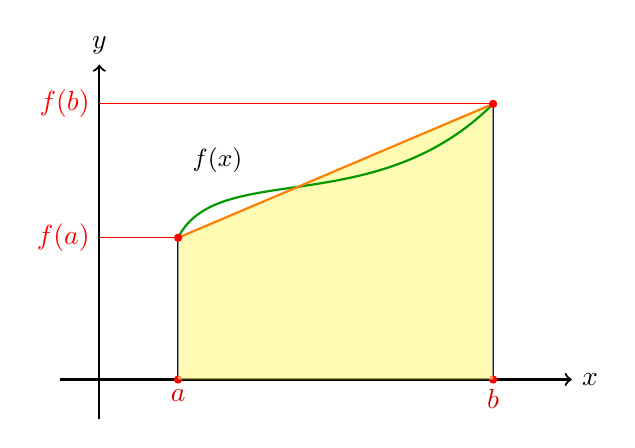
\begin{tikzpicture}
    % Assi
    \draw[thick, ->] (-0.5, 0) -- (6, 0) node[right] {$x$};
    \draw[thick, ->] (0, -0.5) -- (0, 4) node[above] {$y$};
    
    % Nodi e linee verticali
    \draw[blue!80!black, thick] (1, 0) -- (1, 1.8);
    \draw[blue!80!black, thick] (5, 0) -- (5, 3.5);
    \fill[red] (1,0) circle (1.5pt) node[below, text=red!80!black] {$a$};
    \fill[red] (5,0) circle (1.5pt) node[below, text=red!80!black] {$b$};
    
    % Area del trapezio evidenziata
    \fill[yellow!50, opacity=0.6] (1,0) -- (1,1.8) -- (5,3.5) -- (5,0) -- cycle;
    
    % Funzione f(x) (curva verde)
    \draw[thick, green!60!black] (1, 1.8) .. controls (1.5, 2.8) and (3.5, 2.0) .. (5, 3.5);
    
    % Retta secante (arancione)
    \draw[thick, orange] (1, 1.8) -- (5, 3.5);
    
    % Punti e proiezioni su y
    \fill[red] (1, 1.8) circle (1.5pt);
    \fill[red] (5, 3.5) circle (1.5pt);
    \draw[red, thin] (1, 1.8) -- (0, 1.8) node[left] {$f(a)$};
    \draw[red, thin] (5, 3.5) -- (0, 3.5) node[left] {$f(b)$};
    
    % Etichette
    \node[above, font=\small] at (1.5, 2.5) {$f(x)$};
\end{tikzpicture}
\end{center}

In definitiva, approssimiamo l'area sottesa dal grafico di $f(x)$ con l'area del trapezio rettangolo individuato dai punti $(a,0), (b,0), (b,f(b))$ e $(a,f(a))$. Per questo motivo si parla di \textbf{metodo dei trapezi}.

\paragraph{Caso $n=2$ (Metodo di Simpson):}
Dalla \eqref{eq:simmetria_pesi_NC} otteniamo che $c_{02} = c_{22}$, e dalla \eqref{eq:somma_pesi_NC} abbiamo $\frac{1}{2}(c_{02} + c_{12} + c_{22}) = 1 \implies c_{02} + c_{12} + c_{22} = 2$.
Pertanto, calcolando ad esempio $c_{22}$, possiamo ottenere tutti gli altri pesi:
\begin{align*}
c_{22} &= \int_{0}^{2} \frac{t-0}{2-0} \cdot \frac{t-1}{2-1} dt = \int_{0}^{2} \frac{t}{2}(t-1) dt \\
&= \int_{0}^{2} \frac{t^2}{2} dt - \int_{0}^{2} \frac{t}{2} dt = \left[ \frac{t^3}{6} \right]_0^2 - \left[ \frac{t^2}{4} \right]_0^2 = \frac{8}{6} - \frac{4}{4} = \frac{4}{3} - 1 = \frac{1}{3}
\end{align*}
Pertanto, $c_{02} = c_{22} = \frac{1}{3}$. Sostituendo si ottiene $c_{12} = 2 - \frac{2}{3} = \frac{4}{3}$.
In questo modo, si ottiene il \textbf{metodo di Simpson} che, considerato che $x_0 = a, x_2 = b$ e $x_1 = \frac{a+b}{2}$, si può scrivere come:
\begin{equation}
I_2(f) = \frac{b-a}{2} \left( \frac{f(a)}{3} + \frac{4}{3} f\left(\frac{a+b}{2}\right) + \frac{f(b)}{3} \right) = \frac{b-a}{6} \left( f(a) + 4f\left(\frac{a+b}{2}\right) + f(b) \right)
\end{equation}


\vspace{0.6cm}
\subsubsection{Analisi di Condizionamento}

\paragraph{Problema Continuo:} Se $\tilde{f}(x)$ è una perturbazione di $f(x)$, vogliamo ottenere una corrispondente maggiorazione per:
\begin{align*}
|I(f) - I(\tilde{f})| &= \left| \int_{a}^{b} f(x)dx - \int_{a}^{b} \tilde{f}(x)dx \right| = \left| \int_{a}^{b} (f(x) - \tilde{f}(x))dx \right| \\
&\le \int_{a}^{b} |f(x) - \tilde{f}(x)|dx \le \int_{a}^{b} ||f - \tilde{f}|| dx = (b-a) ||f - \tilde{f}||
\end{align*}
(dove si è denotato $|| \cdot || = \max_{x \in [a,b]} |\cdot|$).
In conclusione abbiamo ottenuto che:
\begin{equation}
|I(f) - I(\tilde{f})| \le (b-a) \cdot ||f - \tilde{f}||
\end{equation}

Considerato che $|I(f) - I(\tilde{f})|$ è la misura dell'errore sul risultato finale e $||f - \tilde{f}||$ è la misura dell'errore sul dato in ingresso, concludiamo che:
\begin{equation} \label{eq:condizione_continuo}
K = b-a
\end{equation}
è il numero di condizione di $I(f)$.

\paragraph{Problema Discreto:} Conduciamo la stessa analisi per $I_n(f)$ definito dalla \eqref{eq:formula_newton_cotes}:
\begin{align*}
|I_n(f) - I_n(\tilde{f})| &= \frac{b-a}{n} \left| \sum_{i=0}^{n} c_{in} f_i - \sum_{i=0}^{n} c_{in} \tilde{f}_i \right| = \frac{b-a}{n} \left| \sum_{i=0}^{n} c_{in} (f_i - \tilde{f}_i) \right| \\
&\le \frac{b-a}{n} \sum_{i=0}^{n} |c_{in}| \cdot |f_i - \tilde{f}_i| \le \left( \frac{b-a}{n} \sum_{i=0}^{n} |c_{in}| \right) ||f - \tilde{f}||
\end{align*}
Da questo concludiamo, in modo analogo a quanto fatto nel continuo, che:
\begin{equation} \label{eq:condizione_discreto}
K_n = \frac{b-a}{n} \sum_{i=0}^{n} |c_{in}|
\end{equation}
definisce il numero di condizionamento della formula di Newton-Cotes di grado $n$.

A questo punto, osserviamo che il rapporto:
\begin{equation}
\frac{K_n}{K} = \frac{1}{n} \sum_{i=0}^{n} |c_{in}|
\end{equation}
Se $c_{in} \ge 0$, dalla proprietà \eqref{eq:somma_pesi_NC} otteniamo che $\frac{K_n}{K} = 1$.
Diversamente, $\frac{K_n}{K} > 1$.

Si può verificare che la condizione $c_{in} \ge 0$ vale rigorosamente per $n = 1, \dots,7, 9$, mentre il rapporto $\frac{K_n}{K}$ cresce assai rapidamente per $n \ge 10$.
Da quanto esposto, si conclude che le formule di Newton-Cotes sono da utilizzare solo per i valori di $n = 1, \dots,7, 9$.

\begin{figure}[htbp]
    \centering
    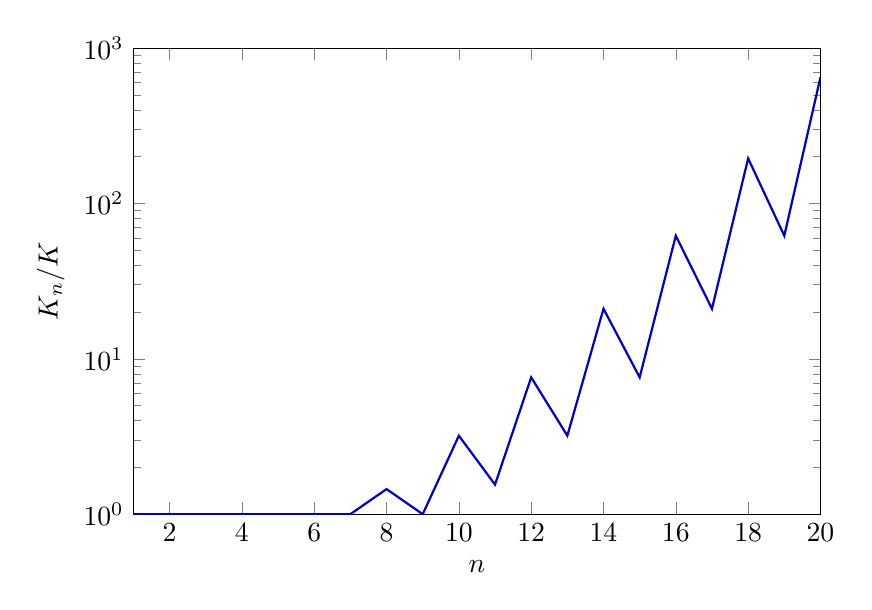
\begin{tikzpicture}
        \begin{semilogyaxis}[
            width=0.85\textwidth, height=7.5cm,
            xmin=1, xmax=20,
            ymin=1, ymax=1000,
            xtick={2,4,6,8,10,12,14,16,18,20},
            ytick={1, 10, 100, 1000},
            yticklabels={$10^0$, $10^1$, $10^2$, $10^3$},
            xlabel={$n$}, 
            ylabel={$K_n / K$},
            axis lines=box,
            grid=none,
            tick align=inside
        ]
            % Andamento reale a zig-zag dei pesi di Newton-Cotes
            \addplot[
                thick, 
                color=blue!80!black,
                mark=none
            ] coordinates {
                (1, 1) (2, 1) (3, 1) (4, 1) (5, 1) (6, 1) (7, 1) 
                (8, 1.45) (9, 1) 
                (10, 3.2) (11, 1.55) 
                (12, 7.6) (13, 3.2) 
                (14, 21) (15, 7.6) 
                (16, 62) (17, 21) 
                (18, 195) (19, 62) 
                (20, 650)
            };
        \end{semilogyaxis}
    \end{tikzpicture}
    \caption{Andamento del rapporto $K_n/K$ al variare di $n$. L'instabilità numerica esplode per $n \ge 10$ con il tipico andamento a zig-zag.}
\end{figure}












%16/04/2026
\vspace{0.6cm}
\subsubsection*{Calcolo pratico dei pesi di Newton-Cotes}

\textbf{OSS:} I coefficienti $c_{in}$ definiti nella formula di Newton-Cotes sono numeri \textbf{razionali}. Infatti:
\begin{equation}
c_{in} = \frac{\alpha_{in}}{d_{in}}
\end{equation}
con:
\begin{equation*}
d_{in} = \prod_{\substack{j=0 \\ j \neq i}}^{n} (i-j) \quad \text{e} \quad \alpha_{in} = \int_{0}^{n} \prod_{\substack{j=0 \\ j \neq i}}^{n} (t-j) dt
\end{equation*}

Possiamo calcolare in Matlab $\alpha_{in}$ e $d_{in}$ facilmente. Per il generico indice $i$, si calcola:
\begin{verbatim}
    ind = [0:i-1, i+1:n];
    din = prod(i - ind);
    a = poly(ind); % coeff. del polinomio monico con le radici
                   % in argomento, per potenze decrescenti.
    \end{verbatim}
    
    Essendo il vettore dei coefficienti:
    \begin{equation*}
    a = [a(1) \quad a(2) \quad \dots \quad a(n+1)]
    \end{equation*}
    ovvero $q(t) = \sum_{i=1}^{n+1} a(i) t^{n+1-i}$, allora il suo integrale è:
    \begin{equation*}
    \int q(t) dt = \sum_{i=1}^{n+1} a(i) \frac{t^{n+2-i}}{n+2-i}
    \end{equation*}
    che è un polinomio omogeneo di grado $n+1$. Completiamo quindi lo script definendo l'array \texttt{q} con i coefficienti della primitiva:
    \begin{verbatim}
    q = [a ./ (n+1:-1:1), 0];
    alfain = polyval(q, n);
    cin = alfain / din;
    format rat
    \end{verbatim}

\vspace{0.6cm}
% --- INIZIO SEZIONE 5.2 DELL'INDICE ---
\subsection{Errore e formule composite}

In questo caso, poiché in generale $I(f) \neq I_n(f)$, vogliamo ottenere un'espressione per l'errore di quadratura:
\begin{equation} \label{eq:errore_quadratura_def}
    \begin{split}
    E_n(f) &= I(f) - I_n(f) = \int_{a}^{b} f(x) dx - \int_{a}^{b} p(x) dx = \int_{a}^{b} (f(x) - p(x)) dx \\[2ex]
    &= \int_{a}^{b} f[x_0, x_1, \dots, x_n, x] \overbrace{\omega_{n+1}(x)}^{= \prod_{i=0}^{n} (x-x_i)} dx
    \end{split}
\end{equation}
dove $p(x)$ è il polinomio interpolante. 
Se assumiamo che $f \in \mathcal{C}^{(n+\mu)}[a,b]$, senza addentrarci nella dimostrazione, si ottiene:
\begin{equation} \label{eq:errore_quadratura_teo}
E_n(f) = \nu_n f^{(n+\mu)}(\xi) \left( \frac{b-a}{n} \right)^{n+\mu+1}
\end{equation}
dove $\nu_n$ è un coefficiente che dipende solo da $n$, $\xi \in (a,b)$, e:
\begin{equation}
\mu = 
\begin{cases} 
1 & \text{se } n \text{ è dispari} \\ 
2 & \text{se } n \text{ è pari} 
\end{cases}
\end{equation}
\textbf{OSS:} Dalla \eqref{eq:errore_quadratura_teo} otteniamo che per far tendere $E_n(f) \to 0$ dovremmo far tendere $n \to \infty$. D'altronde, questo è precluso dal fatto che, per il problema del condizionamento visto in precedenza, richiedevamo $n \in $ \{1,...,7,9\}. Pertanto, abbiamo requisiti contrastanti.

Per ovviare a questo problema, utilizziamo le formule di Newton-Cotes come \textbf{formule composite}.

\vspace{0.6cm}
\subsubsection*{Formule di Quadratura Composite}

Per illustrare questa idea, utilizziamo la formula dei trapezi.

\begin{figure}[htbp]
    \centering
    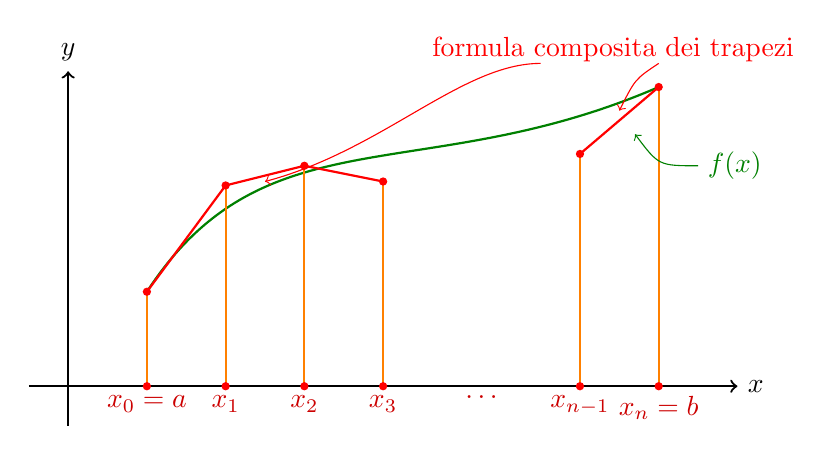
\begin{tikzpicture}
        % Assi
        \draw[thick, ->] (-0.5, 0) -- (8.5, 0) node[right] {$x$};
        \draw[thick, ->] (0, -0.5) -- (0, 4) node[above] {$y$};
        
        % Curve f(x) (verde)
        \draw[thick, green!50!black] (1, 1.2) .. controls (2.5, 3.5) and (4.5, 2.5) .. (7.5, 3.8);
        
        % Nodi verticali (arancioni) e punti rossi
        \foreach \x/\y in {1/1.2, 2/2.55, 3/2.8, 4/2.6, 6.5/2.95, 7.5/3.8} {
            \draw[orange, thick] (\x, 0) -- (\x, \y);
            \fill[red] (\x, \y) circle (1.5pt);
            \fill[red] (\x, 0) circle (1.5pt);
        }
        
        % Etichette asse x
        \node[below, text=red!80!black] at (1,0) {$x_0=a$};
        \node[below, text=red!80!black] at (2,0) {$x_1$};
        \node[below, text=red!80!black] at (3,0) {$x_2$};
        \node[below, text=red!80!black] at (4,0) {$x_3$};
        \node[below, text=red!80!black] at (5.25,0) {$\dots$};
        \node[below, text=red!80!black] at (6.5,0) {$x_{n-1}$};
        \node[below, text=red!80!black] at (7.5,0) {$x_n=b$};
        
        % Trapezi (Linee rosse di congiunzione)
        \draw[thick, red] (1, 1.2) -- (2, 2.55) -- (3, 2.8) -- (4, 2.6);
        \draw[thick, red] (6.5, 2.95) -- (7.5, 3.8);
        
        % Testi e frecce descrittive
        \node[right, green!50!black] at (8, 2.8) {$f(x)$};
        \draw[->, green!50!black] (8, 2.8) .. controls (7.5, 2.8) .. (7.2, 3.2);
        
        \node[above right, red] at (4.5, 4) {formula composita dei trapezi};
        \draw[->, red] (6, 4.1) .. controls (5, 4.1) and (4, 3) .. (2.5, 2.6);
        \draw[->, red] (7.5, 4.1) .. controls (7.2, 3.9) .. (7, 3.5);
        
    \end{tikzpicture}
    \caption{Interpretazione geometrica della formula composita dei trapezi.}
\end{figure}

L'idea in definitiva è la seguente:
\begin{equation} \label{eq:integrale_spezzato}
I(f) = \int_{a}^{b} f(x) dx = \sum_{i=1}^{n} \int_{x_{i-1}}^{x_i} f(x) dx
\end{equation}
Approssimando ogni singolo integrale con la formula dei trapezi, otteniamo:
\begin{equation} \label{eq:composita_trapezi}
 \approx \sum_{i=1}^{n} \frac{b-a}{n} \left( \frac{f_{i-1} + f_i}{2} \right) = \frac{b-a}{n} \sum_{i=1}^{n} \frac{f_{i-1} + f_i}{2} \equiv I_1^{(n)}(f) \text{ (formula composita dei trapezi) }
\end{equation}

Esaminiamo l'errore:
\begin{align*}
E_1^{(n)}(f) &= I(f) - I_1^{(n)}(f) \\
&= \sum_{i=1}^{n} \int_{x_{i-1}}^{x_i} f(x) dx - \frac{b-a}{n} \frac{(f_{i-1} + f_i)}{2} \\
&= \sum_{i=1}^{n} \nu_1 f^{(2)}(\xi_i) \left( \frac{b-a}{n} \right)^3 \quad \text{con } \xi_i \in [x_{i-1}, x_i] \\
&= \nu_1 \left( \frac{b-a}{n} \right)^3 \sum_{i=1}^{n} f^{(2)}(\xi_i)
\end{align*}
Per il teorema della media, la sommatoria è pari a $n \cdot f^{(2)}(\xi)$ con $\xi \in (a,b)$. Quindi:
\begin{equation} \label{eq:errore_composita_trapezi_finale}
E_1^{(n)}(f) = \nu_1 \left( \frac{b-a}{n} \right)^3 n \cdot f^{(2)}(\xi) = \nu_1 (b-a) f^{(2)}(\xi) \left( \frac{b-a}{n} \right)^2 \xrightarrow{n \to \infty} 0
\end{equation}

In generale, se la formula ha grado k ($k \in$ \{ 1,...,7,9\}) e $n$ è un multiplo di $k$ ($n = k \cdot l$), otteniamo che la formula composita di grado $k$ sugli $n+1$ punti $x_i = a+ih$, con $i=0,\dots, n$, $h=\frac{b-a}{n}$, si ottiene applicandola $l$ volte per ricoprire l'intervallo $[a,b]$:
\begin{equation*}
[x_0, x_k] \cup [x_{k+1}, x_{2k}] \cup \dots \cup [x_{k(l-1)}, x_{kl}] = [a,b]
\end{equation*}
In questo modo, il corrispondente errore si vede essere:
\begin{equation} \label{eq:errore_composita_generale}
\begin{split}
E_k^{(n)}(f) &= I(f) - I_k^{(n)}(f) \\[1ex]
&= \nu_k f^{(k+\mu)}(\xi) \cdot l \cdot h^{k+\mu+1}, \quad \xi \in [a,b] \\[1ex]
&= \nu_k f^{(k+\mu)}(\xi) \cdot l \left( \frac{b-a}{n} \right)^{k+\mu+1}, \quad n = kl \\[1ex]
&= \nu_k \frac{(b-a)}{k} f^{(k+\mu)}(\xi) \left( \frac{b-a}{n} \right)^{k+\mu} \xrightarrow{n \to \infty} 0
\end{split}
\end{equation}

\vspace{0.6cm}
\subsubsection*{Esempi di Formule Composite}

\paragraph{$k=1$ (Formula composita dei Trapezi):}
\begin{align} \label{eq:trapezi_esplicita}
I_1^{(n)}(f) &= \frac{b-a}{n} \left( \frac{f_0}{2} + \frac{f_1}{2} + \frac{f_1}{2} + \frac{f_2}{2} + \dots + \frac{f_{n-1}}{2} + \frac{f_n}{2} \right) \nonumber \\
&= \frac{b-a}{n} \left( \frac{f_0}{2} + \sum_{i=1}^{n-1} f_i + \frac{f_n}{2} \right)
\end{align}
\textbf{OSS:} Se $f$ è periodica in $[a,b] \implies f_0 = f_n$, da cui $I_1^{(n)}(f) = \frac{b-a}{n} \sum f_i$ (N.B. essenziale nella elaborazione numerica dei segnali).

\paragraph{$k=2$ (Formula composita di Simpson):}
In questo caso $n$ deve essere pari ($n = 2l$). Si ottiene:
\begin{align} \label{eq:simpson_esplicita}
I_2^{(n)}(f) &= \frac{b-a}{n} \left[ \frac{f_0 + 4f_1 + f_2}{3} + \frac{f_2 + 4f_3 + f_4}{3} + \dots + \frac{f_{n-2} + 4f_{n-1} + f_n}{3} \right] \nonumber \\
&= \frac{b-a}{3n} \left[ 4\sum_{i=1}^{n/2} f_{2i-1} + 2\sum_{i=0}^{n/2} f_{2i} - f_0 - f_n \right]
\end{align}

\vspace{0.6cm}
\textbf{N.B.} In ogni caso, tutti i valori di $f$ necessari possono essere precalcolati (possibilmente in modo vettoriale) come segue:
\begin{verbatim}
x = linspace(a, b, n+1); % punti xi
f = fun(x);
\end{verbatim}
Sia \texttt{fun} la function che implementa la funzione integranda. Il comando restituisce pertanto tutti i valori della funzione integranda richiesti per implementare la formula composita in esame. Bisogna \textbf{evitare valutazioni funzionali ridondanti}.

\vspace{0.6cm}
\paragraph{Esempio Numerico:}
Consideriamo l'approssimazione di questo integrale:
\begin{equation}
I(f) = \int_{0}^{\pi} \sin(x) dx = 2
\end{equation}

\begin{table}[htbp]
\centering
\renewcommand{\arraystretch}{1.2}
\begin{tabular}{ccccc}
\toprule
$n$ & $I_1^{(n)}$ & $E_1^{(n)}$ & $I_2^{(n)}$ & $E_2^{(n)}$ \\
\midrule
2  & 1.5708 & $4.2920 \cdot 10^{-1}$ & 2.0944 & $-9.4395 \cdot 10^{-2}$ \\
4  & 1.8961 & $1.0388 \cdot 10^{-1}$ & 2.0046 & $-4.5598 \cdot 10^{-3}$ \\
6  & 1.9541 & $4.5903 \cdot 10^{-2}$ & 2.0009 & $-8.6319 \cdot 10^{-4}$ \\
8  & 1.9742 & $2.5768 \cdot 10^{-2}$ & 2.0003 & $-2.6917 \cdot 10^{-4}$ \\
10 & 1.9835 & $1.6476 \cdot 10^{-2}$ & 2.0001 & $-1.0952 \cdot 10^{-4}$ \\
12 & 1.9886 & $1.1436 \cdot 10^{-2}$ & 2.0001 & $-5.2624 \cdot 10^{-5}$ \\
14 & 1.9916 & $8.3996 \cdot 10^{-3}$ & 2.0000 & $-2.8344 \cdot 10^{-5}$ \\
16 & 1.9936 & $6.4297 \cdot 10^{-3}$ & 2.0000 & $-1.6591 \cdot 10^{-5}$ \\
18 & 1.9949 & $5.0795 \cdot 10^{-3}$ & 2.0000 & $-1.0348 \cdot 10^{-5}$ \\
20 & 1.9959 & $4.1140 \cdot 10^{-3}$ & 2.0000 & $-6.7844 \cdot 10^{-6}$ \\
\bottomrule
\end{tabular}
\end{table}













%22/04/2026
\vspace{0.6cm}
\subsubsection*{Stima dell'errore di quadratura}

Vediamo se dalla formula dell'errore si possa ottenere, a costo nullo, una stima dell'errore di quadratura.

\textbf{OSS:} il costo computazionale verrà misurato in termini di valutazioni funzionali della funzione integranda, che, pertanto, non devono essere ridondanti.

Supponiamo che, nella formula composita, $n$ sia un multiplo pari di $k$, ovvero $n = 2kl$. Allora possiamo applicare la formula composita sia su tutti gli $n+1$ punti, che solo su quelli di indice pari.

\begin{center}
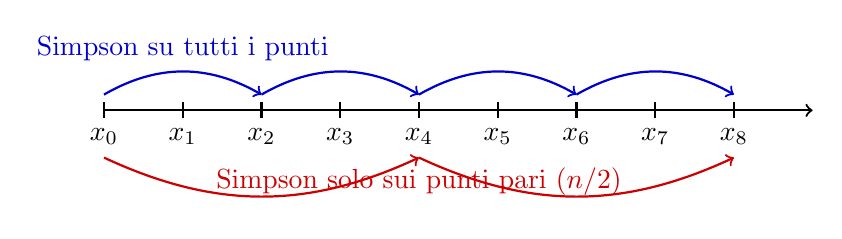
\begin{tikzpicture}
    % Linea base
    \draw[thick, ->] (0,0) -- (9,0);
    
    % Nodi
    \foreach \x/\i in {0/0, 1/1, 2/2, 3/3, 4/4, 5/5, 6/6, 7/7, 8/8} {
        \draw[thick] (\x, 0.1) -- (\x, -0.1) node[below] {$x_{\i}$};
    }
    
    % Archi per Simpson (k=2)
    \node[above, text=blue!80!black] at (1, 0.5) {Simpson su tutti i punti};
    \draw[->, thick, blue!80!black] (0, 0.2) to[bend left=30] (2, 0.2);
    \draw[->, thick, blue!80!black] (2, 0.2) to[bend left=30] (4, 0.2);
    \draw[->, thick, blue!80!black] (4, 0.2) to[bend left=30] (6, 0.2);
    \draw[->, thick, blue!80!black] (6, 0.2) to[bend left=30] (8, 0.2);
    
    % Archi per Simpson sui punti pari
    \node[above, text=red!80!black] at (4, -1.2) {Simpson solo sui punti pari ($n/2$)};
    \draw[->, thick, red!80!black] (0, -0.6) to[bend right=25] (4, -0.6);
    \draw[->, thick, red!80!black] (4, -0.6) to[bend right=25] (8, -0.6);
\end{tikzpicture}
\end{center}

Così facendo, dalla formula generale dell'errore otteniamo che per un opportuno $\hat{\xi} \in [a,b]$ (generalmente $\hat{\xi} \neq \xi$) e ponendo $n/2$ al posto di $n$ (poiché l'intervallo è doppio, il passo è $2h$):
\begin{equation} \label{eq:errore_n_mezzi}
I(f) - I_k^{(n/2)}(f) = \nu_k \left(\frac{b-a}{k}\right) f^{(k+\mu)}(\hat{\xi}) \left(\frac{b-a}{n/2}\right)^{k+\mu}
\end{equation}
Ricordiamo inoltre la formula per $n$ intervalli:
\begin{equation} \label{eq:errore_n_intero}
I(f) - I_k^{(n)}(f) = \nu_k \left(\frac{b-a}{k}\right) f^{(k+\mu)}(\xi) \left(\frac{b-a}{n}\right)^{k+\mu}
\end{equation}

Facendo l'assunzione che $\hat{\xi} \approx \xi$ e sottraendo la \eqref{eq:errore_n_intero} dalla \eqref{eq:errore_n_mezzi} membro a membro, otteniamo:
\begin{equation*}
I_k^{(n)}(f) - I_k^{(n/2)}(f) \approx \nu_k \left(\frac{b-a}{k}\right) f^{(k+\mu)}(\xi) \left(\frac{b-a}{n}\right)^{k+\mu} (2^{k+\mu} - 1)
\end{equation*}

Pertanto, dividendo membro a membro per $2^{k+\mu} - 1$, otteniamo l'espressione per la stima dell'errore:
\begin{equation} \label{eq:stima_errore_quad}
\hat{E}_k^{(n)}(f) = \frac{I_k^{(n)}(f) - I_k^{(n/2)}(f)}{2^{k+\mu} - 1} \approx \nu_k \left(\frac{b-a}{k}\right) f^{(k+\mu)}(\xi) \left(\frac{b-a}{n}\right)^{k+\mu} = I(f) - I_k^{(n)}(f) = E_k^{(n)}(f)
\end{equation}

Così facendo, otteniamo una stima computazionale dell'errore di quadratura. Chiaramente, questa stima diviene più accurata al crescere di $n$.

Ad esempio, se consideriamo l'integrale $I(f) = \int_{0}^{\pi} \sin(x) dx = 2$ ed utilizziamo le formule composite dei trapezi e di Simpson ($k=1$ e $k=2$, rispettivamente), si ottiene la seguente tabella comparativa tra l'errore reale $E$ e la stima $\hat{E}$:

\begin{table}[htbp]
\centering
\renewcommand{\arraystretch}{1.2}
\small
\begin{tabular}{ccccccc}
\toprule
$n$ & $I_1^{(n)}$ & $E_1^{(n)}$ & $\hat{E}_1^{(n)}$ & $I_2^{(n)}$ & $E_2^{(n)}$ & $\hat{E}_2^{(n)}$ \\
\midrule
2 & 1.5708 & $4.2920 \cdot 10^{-1}$ & $5.2360 \cdot 10^{-1}$ & 2.0944 & $-9.4395 \cdot 10^{-2}$ & - \\
4 & 1.8961 & $1.0388 \cdot 10^{-1}$ & $1.0844 \cdot 10^{-1}$ & 2.0046 & $-4.5598 \cdot 10^{-3}$ & $-5.9890 \cdot 10^{-3}$ \\
6 & 1.9541 & $4.5903 \cdot 10^{-2}$ & $4.6766 \cdot 10^{-2}$ & 2.0009 & $-8.6319 \cdot 10^{-4}$ & - \\
8 & 1.9742 & $2.5768 \cdot 10^{-2}$ & $2.6038 \cdot 10^{-2}$ & 2.0003 & $-2.6917 \cdot 10^{-4}$ & $-2.8604 \cdot 10^{-4}$ \\
10 & 1.9835 & $1.6476 \cdot 10^{-2}$ & $1.6586 \cdot 10^{-2}$ & 2.0001 & $-1.0952 \cdot 10^{-4}$ & - \\
12 & 1.9886 & $1.1436 \cdot 10^{-2}$ & $1.1489 \cdot 10^{-2}$ & 2.0001 & $-5.2624 \cdot 10^{-5}$ & $-5.4038 \cdot 10^{-5}$ \\
14 & 1.9916 & $8.3996 \cdot 10^{-3}$ & $8.4279 \cdot 10^{-3}$ & 2.0000 & $-2.8344 \cdot 10^{-5}$ & - \\
16 & 1.9936 & $6.4297 \cdot 10^{-3}$ & $6.4462 \cdot 10^{-3}$ & 2.0000 & $-1.6591 \cdot 10^{-5}$ & $-1.6839 \cdot 10^{-5}$ \\
18 & 1.9949 & $5.0795 \cdot 10^{-3}$ & $5.0899 \cdot 10^{-3}$ & 2.0000 & $-1.0348 \cdot 10^{-5}$ & - \\
20 & 1.9959 & $4.1140 \cdot 10^{-3}$ & $4.1208 \cdot 10^{-3}$ & 2.0000 & $-6.7844 \cdot 10^{-6}$ & $-6.8489 \cdot 10^{-6}$ \\
\bottomrule
\end{tabular}
\end{table}


\vspace{0.8cm}
% --- INIZIO SEZIONE 5.3 DELL'INDICE ---
\subsection{Formule adattative}

Possiamo specializzare ulteriormente questa stima dell'errore di quadratura, per ottenere delle formule di quadratura di tipo adattivo.

Il problema è il seguente: talora la funzione integranda ha un comportamento che è variabile (talora anche molto) in sottointervalli dell'intervallo di integrazione. In questo caso può essere conveniente utilizzare dei punti distribuiti non uniformemente, ma adattati al comportamento locale di $f(x)$. Il fine è, pertanto, quello di soddisfare un prescritto criterio di accuratezza con un numero di punti minore possibile.

\textbf{Esempio:}
\begin{equation}
\int_{1/2}^{100} -2x^{-3}\cos(x^{-2})dx \equiv \sin(10^{-4}) - \sin(4)
\end{equation}

\begin{figure}[htbp]
    \centering
    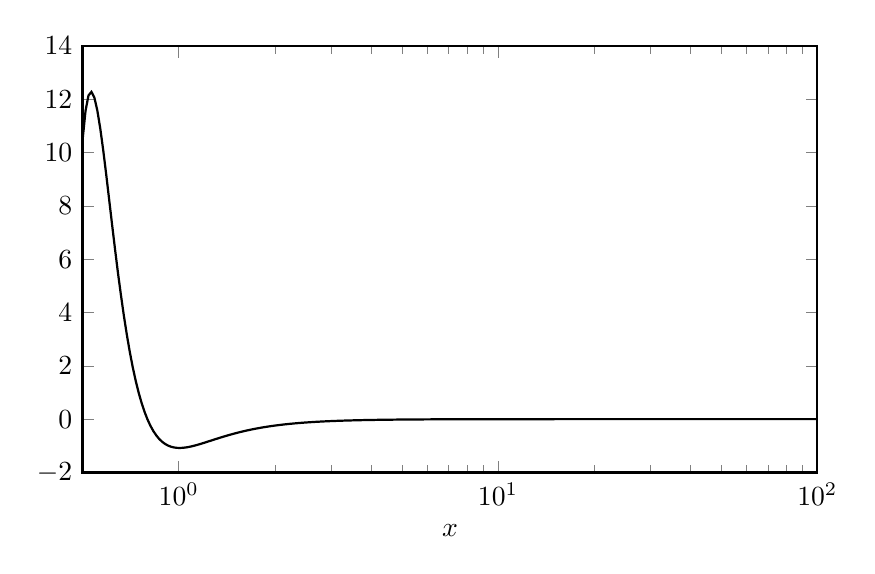
\begin{tikzpicture}
        \begin{semilogxaxis}[
            width=0.9\textwidth, height=7cm,
            xmin=0.5, xmax=100,
            ymin=-2, ymax=14,
            xlabel={$x$},
            xtick={1, 10, 100},
            ytick={-2, 0, 2, 4, 6, 8, 10, 12, 14},
            axis lines=box,
            tick align=inside,
            thick
        ]
            \addplot[thick, color=black, samples=250, domain=0.5:100] {-2*x^(-3)*cos(deg(x^(-2)))};
        \end{semilogxaxis}
    \end{tikzpicture}
    \caption{Comportamento fortemente oscillante della funzione vicino all'origine.}
\end{figure}

Illustriamo questo concetto con la formula dei trapezi, di cui esaminiamo una facile implementazione, sebbene la procedura si estenda facilmente al caso di formule di base più accurate.

\textbf{Problema:} calcolare $I(f)$ con una tolleranza \texttt{tol} prescritta.

Applicando la formula dei trapezi su [a,b] e quella composita con $n=2$ otteniamo che:
\begin{align*}
I_1 &= \frac{b-a}{2}(f(a) + f(b)) \\
I_2 &= \frac{b-a}{4}(f(a) + 2f(x_1) + f(b)) \quad \text{con } x_1 = \frac{a+b}{2}
\end{align*}

Abbiamo visto che la stima dell'errore è ottenibile come (essendo per i trapezi $k=1, \mu=1 \implies 2^{1+1}-1 = 3$):
\begin{equation*}
E_{12} = \frac{|I_2 - I_1|}{3}
\end{equation*}

A questo punto:
\begin{enumerate}
    \item Se $E_{12} \le \text{tol}$, ho finito $\implies I_2$
    \item Altrimenti, riapplico la stessa procedura su $[a, x_1]$ e $[x_1, b]$ con tolleranza $\text{tol}/2$.
\end{enumerate}

L'accortezza nell'implementare questa procedura è quella di \textbf{evitare valutazioni funzionali ridondanti} della funzione integranda. Infatti, nel caso 2 abbiamo già calcolato $f(a)$, $f(x_1)$ e $f(b)$ che, pertanto, non andranno ricalcolati.

Ad esempio, per l'integrale visto in precedenza, con tolleranza prescritta (tol = $10^{-3}$), l'algoritmo adattivo concentra i punti di valutazione laddove la funzione varia maggiormente (vicino all'origine):

\begin{figure}[htbp]
    \centering
    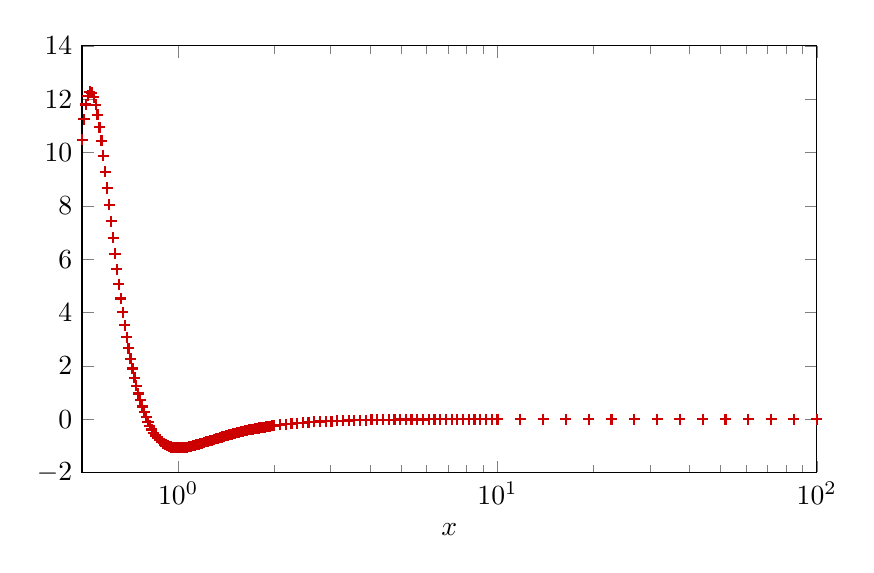
\begin{tikzpicture}
        \begin{semilogxaxis}[
            width=0.9\textwidth, height=7cm,
            xmin=0.5, xmax=100,
            ymin=-2, ymax=14,
            xlabel={$x$},
            xtick={1, 10, 100},
            ytick={-2, 0, 2, 4, 6, 8, 10, 12, 14},
            axis lines=box,
            tick align=inside
        ]
            % Simulazione della densità dei nodi adattivi: fitti a sinistra, sparsi a destra
            \addplot[only marks, mark=+, draw=red!80!black, thick, samples=100, domain=0.5:2] {-2*x^(-3)*cos(deg(x^(-2)))};
            \addplot[only marks, mark=+, draw=red!80!black, thick, samples=40, domain=2:10] {-2*x^(-3)*cos(deg(x^(-2)))};
            \addplot[only marks, mark=+, draw=red!80!black, thick, samples=15, domain=10:100] {-2*x^(-3)*cos(deg(x^(-2)))};
        \end{semilogxaxis}
    \end{tikzpicture}
    \caption{Distribuzione dei punti di quadratura adattiva: si infittiscono dove la funzione è più critica.}
\end{figure}

Mediante una semplice implementazione in Matlab, lo script risultante è il seguente:

\begin{verbatim}
function I2 = trapead(fun, a, b, tol, fa, fb)
% I2 = trapead(fun, a, b, tol)
% Calcolo l'integrale di fun in [a,b] con tolleranza tol
%
% < Controlli di consistenza >

if nargin == 4
    fa = fun(a);
    fb = fun(b);
end

x1 = (a+b)/2;
f1 = fun(x1);
h = (b-a)/2;

I1 = (fa+fb)*h;
I2 = (fa+2*f1+fb)*h/2;
err = abs(I2-I1)/3;

if err > tol
    I2 = trapead(fun, a, x1, tol/2, fa, f1) + ...
         trapead(fun, x1, b, tol/2, f1, fb);
end

return
\end{verbatim}